
\documentclass[11pt,fleqn]{article} 
\usepackage[margin=0.8in, head=0.8in]{geometry} 
\usepackage{amsmath, amssymb, amsthm}
\usepackage{fancyhdr} 
\usepackage{palatino, url, multicol}
\usepackage{graphicx, pgfplots} 
\usepackage[all]{xy}
\usepackage{polynom} 
\usepackage{enumerate}
\usepackage{framed}
\usepackage{setspace}
\usepackage{array,tikz}

\pgfplotsset{compat=1.6}

\pgfplotsset{soldot/.style={color=black,only marks,mark=*}} \pgfplotsset{holdot/.style={color=black,fill=white,minimum size=10mm,only marks,mark=*}}


\pagestyle{fancy} 
\rfoot{2-2 The Limit of a Function}

\begin{document}
\renewcommand{\headrulewidth}{0pt}
\newcommand{\blank}[1]{\rule{#1}{0.75pt}}
\newcommand{\bc}{\begin{center}}
\newcommand{\ec}{\end{center}}
\renewcommand{\d}{\displaystyle}

\vspace*{-0.7in}

%%%%%%%%%intro page
\begin{center}
  \LARGE
  \sc{Section 2-2: The Limit of a Function}\\
\end{center}
Read Section 2.2. Work the embedded problems. \\
Goals: \\
\begin{itemize}
	\item Understand the meaning of the notation $\d \lim_{x \to a} f(x)=L$.
	\item Know how to evaluate one- and two-sided limits both from a graph and numerically.
	\item Understand the relationship between infinite limits and vertical asymptotes.
\end{itemize}
\begin{enumerate}
\item \fbox{{\sc{definition:}}} \textbf{two-sided limit}\\

Notation: \\

Words: \\

It means: \\
\vspace{0.5in}

\item Evaluate the limits below using the graph and confirm your answers numerically.\\

\begin{tabular}{lll}
(a) $f(x)=\frac{x^2-4}{x-2}$\quad\hspace{1in}\quad&(b) $f(x)=\frac{|x-2|}{x-2}$\quad\hspace{1in}\quad&(c) $f(x)=\frac{1}{(x-2)^2}$\\
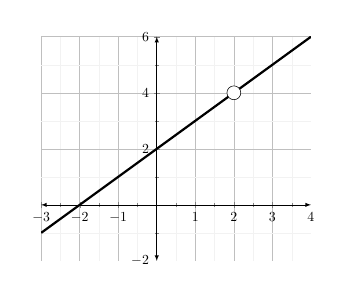
\begin{tikzpicture}[scale=0.5]
\begin{axis}[grid style={line width=.2pt, draw=gray!10},grid=both,major grid style={line width=.4pt,draw=gray!50},
    xmin=-3,xmax=4,
    ymin=-2,ymax=6,
    xtick={},ytick={},
    minor tick num=1,
    axis lines=middle, mark size=5.0pt,
    enlargelimits={abs=0},
    axis line style={latex-latex},
    xlabel style={at={(ticklabel* cs:1)},anchor=north west},
    ylabel style={at={(ticklabel* cs:1)},anchor=south west}]
\addplot[domain=-3:4, black,ultra thick, smooth] {x+2};
\addplot[mark=*,fill=white,only marks, ] coordinates {(2,4)};
\end{axis}
\end{tikzpicture}
&
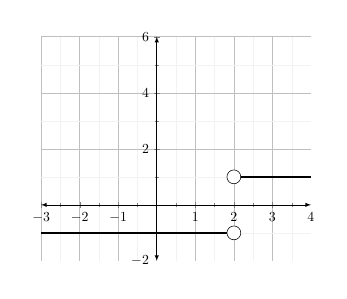
\begin{tikzpicture}[scale=0.5]
\begin{axis}[grid style={line width=.2pt, draw=gray!10},grid=both,major grid style={line width=.4pt,draw=gray!50},
    xmin=-3,xmax=4,
    ymin=-2,ymax=6,
    xtick={},ytick={},
    minor tick num=1,
    axis lines=middle, mark size=5.0pt,
    enlargelimits={abs=0},
    axis line style={latex-latex},
    xlabel style={at={(ticklabel* cs:1)},anchor=north west},
    ylabel style={at={(ticklabel* cs:1)},anchor=south west}]
\addplot[domain=-3:2, black,ultra thick, smooth] {-1};
\addplot[domain=2:4, black,ultra thick, smooth] {1};
\addplot[mark=*,fill=white,only marks] coordinates {(2,1) (2,-1)};
\end{axis}
\end{tikzpicture}
&
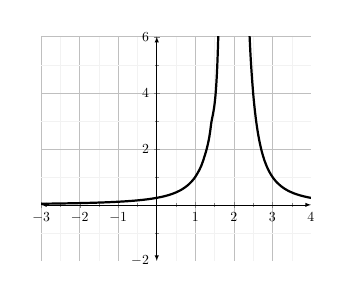
\begin{tikzpicture}[scale=0.5]
\begin{axis}[grid style={line width=.2pt, draw=gray!10},grid=both,major grid style={line width=.4pt,draw=gray!50},
    xmin=-3,xmax=4,
    ymin=-2,ymax=6,
    xtick={},ytick={},
    minor tick num=1,
    axis lines=middle, mark size=5.0pt,
    enlargelimits={abs=0},
    axis line style={latex-latex},
    xlabel style={at={(ticklabel* cs:1)},anchor=north west},
    ylabel style={at={(ticklabel* cs:1)},anchor=south west}]
\addplot[domain=-3:1.8, black,ultra thick, smooth] {1/((x-2)*(x-2))};
\addplot[domain=2.2:4, black,ultra thick, smooth] {1/((x-2)*(x-2))};\end{axis}
\end{tikzpicture} \\
&&\\ 
graphically:&&\\
&&\\
$\d \lim_{x \to 2}\frac{x^2-4}{x-2}= $ & $\d \lim_{x \to 2} \frac{|x-2|}{x-2}=$ & $\d \lim_{x \to 2} \frac{1}{(x-2)^2}=$\\
&&\\
numerically:&&\\
\end{tabular}
\newpage
\item Numerically or graphically, determine the limits below. Assume $a$ and $c$ are fixed constants.

\begin{enumerate}
\item $\d \lim_{x \to 0} = \frac{\sin(x)}{x}$\\
\vspace{1in}

\begin{multicols}{3}
\item $\d \lim_{x \to 1}  5=$
\item $\d \lim_{x \to 2 } 5=$
\item $\d \lim_{x \to a } c=$
\end{multicols}

\quad

\begin{multicols}{3}
\item $\d \lim_{x \to 1}x =$
\item $\d \lim_{x \to 2} x=$
\item $\d \lim_{x \to a} x=$
\end{multicols}
\quad
\end{enumerate}
\item Return to problem 2b above. Evaluate the limits below assuming that \\

 $x \to 2^-$ means \\
 
 and\\
 
  $x \to 2^+$ means \\
  \begin{multicols}{2}
  \begin{enumerate}
  \item $\d \lim_{x \to 2^-} \frac{|x-2|}{x-2}=$
  \item $\d \lim_{x \to 2^+} \frac{|x-2|}{x-2}=$
  \end{enumerate}
  \end{multicols}
\vfill
\item What must be the relationship between the existence of two-sided limits in terms of one-sided limits?

\vfill
\newpage
\item \fbox{{\sc{definition:}}} infinite limits\\

\vfill

\item The function $g(x)$ is graphed below. Use the graph to fill in the blanks.

\begin{tabular}{m{9cm}  c m{5cm}}
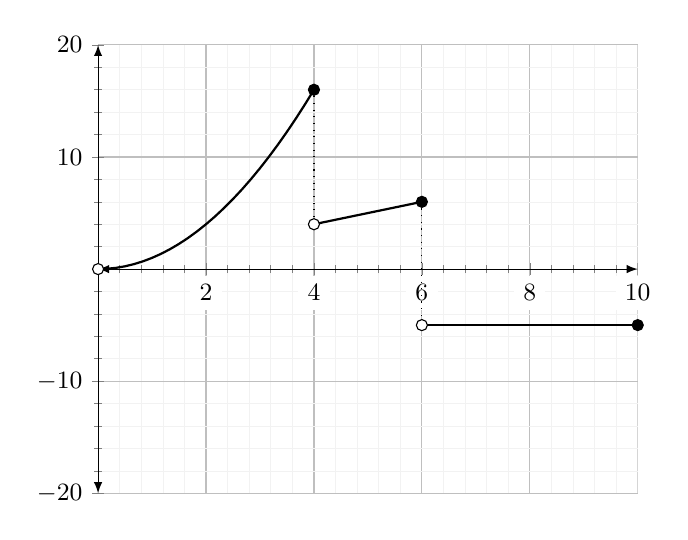
\begin{tikzpicture}[scale=1]
\begin{axis}[grid style={line width=.2pt, draw=gray!10},grid=both,major grid style={line width=.4pt,draw=gray!50},
    xmin=0,xmax=10,
    ymin=-20,ymax=20,
    xtick={},ytick={},
    minor tick num=4,
    enlargelimits={abs=0},
    ticklabel style={font=\small,fill=white},
    axis lines=middle,
    axis line style={latex-latex},
    xlabel style={at={(ticklabel* cs:1)},anchor=north west},
    ylabel style={at={(ticklabel* cs:1)},anchor=south west}
]
\addplot[domain=0:4,black, thick] {x*x};
\addplot[domain=4:6,black, thick] {x};
\addplot[domain=6:10,black, thick] {-5};
\draw[dotted] (axis cs:4,16) -- (axis cs:4,4);
\draw[dotted] (axis cs:6,6) -- (axis cs:6,-5);
\addplot[holdot] coordinates{(0,0)(4,4)(6,-5)};
\addplot[soldot] coordinates{(4,16)(6,6)(10,-5)};
\end{axis}
\end{tikzpicture}
& \quad &
\begin{enumerate}
\item$\d{\lim_{x \to 4^-} f(x) = \underline{\hspace{2cm}} }$
\item$\d{\lim_{x \to 4^+} f(x) = \underline{\hspace{2cm}} }$
\item$\d{\lim_{x \to 4} f(x) = \underline{\hspace{2cm}} }$
\item $f(4)= \underline{\hspace{2cm}}$
\item $\d{\lim_{x \to 8} f(x) = \underline{\hspace{2cm}} }$
\item $f(8)= \underline{\hspace{2cm}}$
\end{enumerate}
\end{tabular}

\item The function $g(x)$ is graphed below. Use the graph to fill in the blanks.

\begin{tabular}{m{9cm}  c m{5cm}}
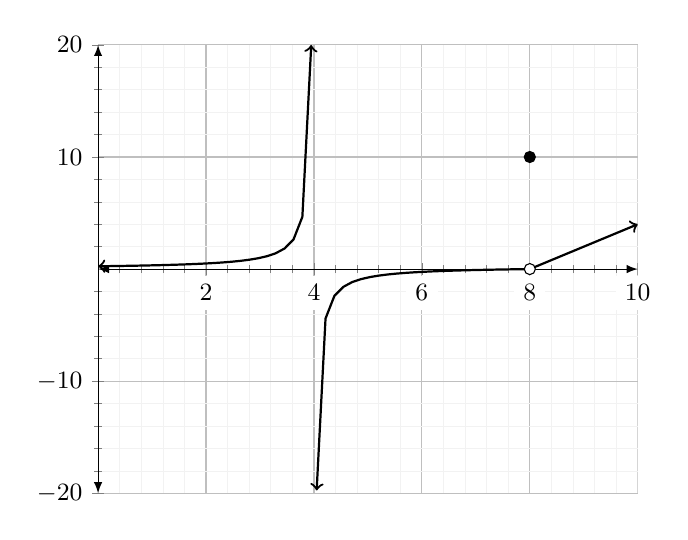
\begin{tikzpicture}[scale=1]
\begin{axis}[grid style={line width=.2pt, draw=gray!10},grid=both,major grid style={line width=.4pt,draw=gray!50},
    xmin=0,xmax=10,
    ymin=-20,ymax=20,
    xtick={},ytick={},
    minor tick num=4,
    enlargelimits={abs=0},
    ticklabel style={font=\small,fill=white},
    axis lines=middle,
    axis line style={latex-latex},
    xlabel style={at={(ticklabel* cs:1)},anchor=north west},
    ylabel style={at={(ticklabel* cs:1)},anchor=south west}
]

\addplot[<->,domain=0:3.95,black, thick] {(4-x)^(-1)};
\addplot[<-,domain=4.05:8,black, thick] {(4-x)^(-1)+0.25};
\addplot[->,domain=8:10,black, thick] {2*x-16};
%\draw[dotted] (axis cs:4,16) -- (axis cs:4,4);
%\draw[dotted] (axis cs:6,6) -- (axis cs:6,-5);
\addplot[soldot] coordinates{(8,10)};
\addplot[holdot] coordinates{(8,0)};
\end{axis}
\end{tikzpicture}
& \quad &
\begin{enumerate}
\item$\d{\lim_{x \to 4^-} f(x) = \underline{\hspace{2cm}} }$
\item$\d{\lim_{x \to 4^+} f(x) = \underline{\hspace{2cm}} }$
\item$\d{\lim_{x \to 4} f(x) = \underline{\hspace{2cm}} }$
\item $f(4)= \underline{\hspace{2cm}}$
\item $\d{\lim_{x \to 8} f(x) = \underline{\hspace{2cm}} }$
\item $f(8)= \underline{\hspace{2cm}}$
\end{enumerate}
\end{tabular}

\newpage
\item Find any vertical asymptotes of $f(x)=\frac{2}{x+5}$ and \emph{justify} your answer using a limit.
\vfill

\item Sketch the graph of an function that satisfies \emph{all} of the given conditions. Compare your answer with that of your neighbor.\\
\begin{tabular}{llll}
&&\\
$\displaystyle{\lim_{x \to 0^-} f(x)=1}$& $\displaystyle{\lim_{x \to 0^+ }f(x)=-2}$ &$\displaystyle{\lim_{x \to 4^-}f(x)=3}$&$\displaystyle{\lim_{x \to 4^+ }f(x)=0}$\\ 
&&\\
 $f(0)=-2$& &$f(4)=1$&\\
\end{tabular}
\vspace{3in}
\end{enumerate}
\end{document}

